\chapter{Methodology}


\section{Simulation Environment}

This section describes the environment and tools used for the experiments.

MuJoCo is a physics engine used to simulate the physical models of the environment. MuJoCo is currently still in development and is improved, so there are many different versions. For this thesis, MuJoCo 2.0 for Linux (Ubuntu 16.04) is used. 
\newline
mujoco-py is used as an interface to allow the usage of MuJoCo in python scripts. mujoco-py is required for OpenAI Gym to work.
\newline
OpenAI developed OpenAI Gym, a toolkit to create and use environments, and use these environments to test and compare algorithms for RL. OpenAI Gym only provides the environment part of RL, the agent has to be written by the user or by using OpenAI baselines. The robotic environments require MuJoCo. In our case, we will create our own environments and compare them to the existing ones.
\newline
OpenAI baselines is a toolkit with high-quality implementations of RL algorithms. It supplements the OpenAI Gym toolkit. For each of the environments by OpenAI Gym, any OpenAI baselines RL algorithm can be used. In our case, we will focus mainly on HER.
\newline
All the experiments will run on a 12 core machine using 10 cores. The machine is running on the operating system Linux Ubuntu 16.04. The parameters used are listed in the appendix. If not otherwise specified, each experiment will be run for 50 episodes. which takes about 2 hours of training time each.


\subsection{MuJoCo}
%physic engine, modeling, mujoco-py for python interface

%mujco is free (no costs) for non-profit research ?
MuJoCo stands for "Multi-Joint dynamics with Contact". It is a physics engine for model based control and was developed by Todorov et al. \cite{mujoco}.
MuJoCo was developed for research in areas with fast and accurate simulation, like robotics. As its name suggests, multi-joint dynamics and contact responses and contact responses are a main focus of the engine. They represented multi-joint dynamics in generalized coordinates and computed them with recursive algorithms. For the contact responses, they wrote algorithms based on a modern velocity-stepping approach. MuJoCo was developed to be fast and accurate, especially for computationally intensive processes, which are common in simulations of physics. 
\newline
Todorov et al. compared MuJoCo to SD/FAST, another tool to simulate physics of mechanical systems. Even though SD/FAST uses model-specific code, which was expected to be much fast, MuJoCo was quite comparable. Their tests with a 12-core machine showed 400.000 dynamics evaluations per second for a 3D humanoid with 18 DOF and 6 active contacts. 
Creating models for MuJoCo is quite simple. For MuJoCo, XML files can be used, which are simple to understand and provide high transparency. 
%explain more how to do xml for mujoco ? - no
\newline
To use MuJoCo with Python, mujoco-py was created by OpenAI. Mujoco-py currently supports compatibility of MuJoCo with Python 3.

\subsection{OpenAI}
Brockman et al. developed OpenAI Gym \cite{gym} and Dhariwal et al. developed OpenAI Baselines \cite{baselines}. Both are freely accessible on Github.

\subsubsection{OpenAI Gym}
%environments
OpenAI Gym provides an environment to test a RL algorithm with. OpenAI Gym already contains many environments to use, like Atari games, classic control problems and robotics. In this thesis, the robotics environment will be used, as it provides four environments with fetch robots that use a robotic arm. But OpenAI also allows the user to create his own environments. For the experiments, a few more robotics environments will be created. For the robotics environments MuJoCo is required. 
The agent and the RL algorithms that are required for RL to interact with the environment have to be either coded by the user or provided by OpenAI Baselines.

\subsubsection{OpenAI Baselines}
%algorithms
OpenAI Baselines provides a set of high-quality implementations of RL algorithms. It can be used together with OpenAI Gym. Provided algorithms contain Advantage Actor Critic, Actor critic with experience replay, Actor Critic using Kronecker-Factored Trust Region, DDPG, Deep Q-Networks, Generative Adversarial Imitation Learning, Proximal Policy Optimization, Trust Region Policy Optimization and HER.
For our purposes, HER in conjunction with DDPG will be used. 
OpenAI Baselines also requires Tensorflow to work.

\section{Model}
%Explain general things like action space etc. of the robot. sucess rate etc.

\begin{figure} [h]
	\centering
	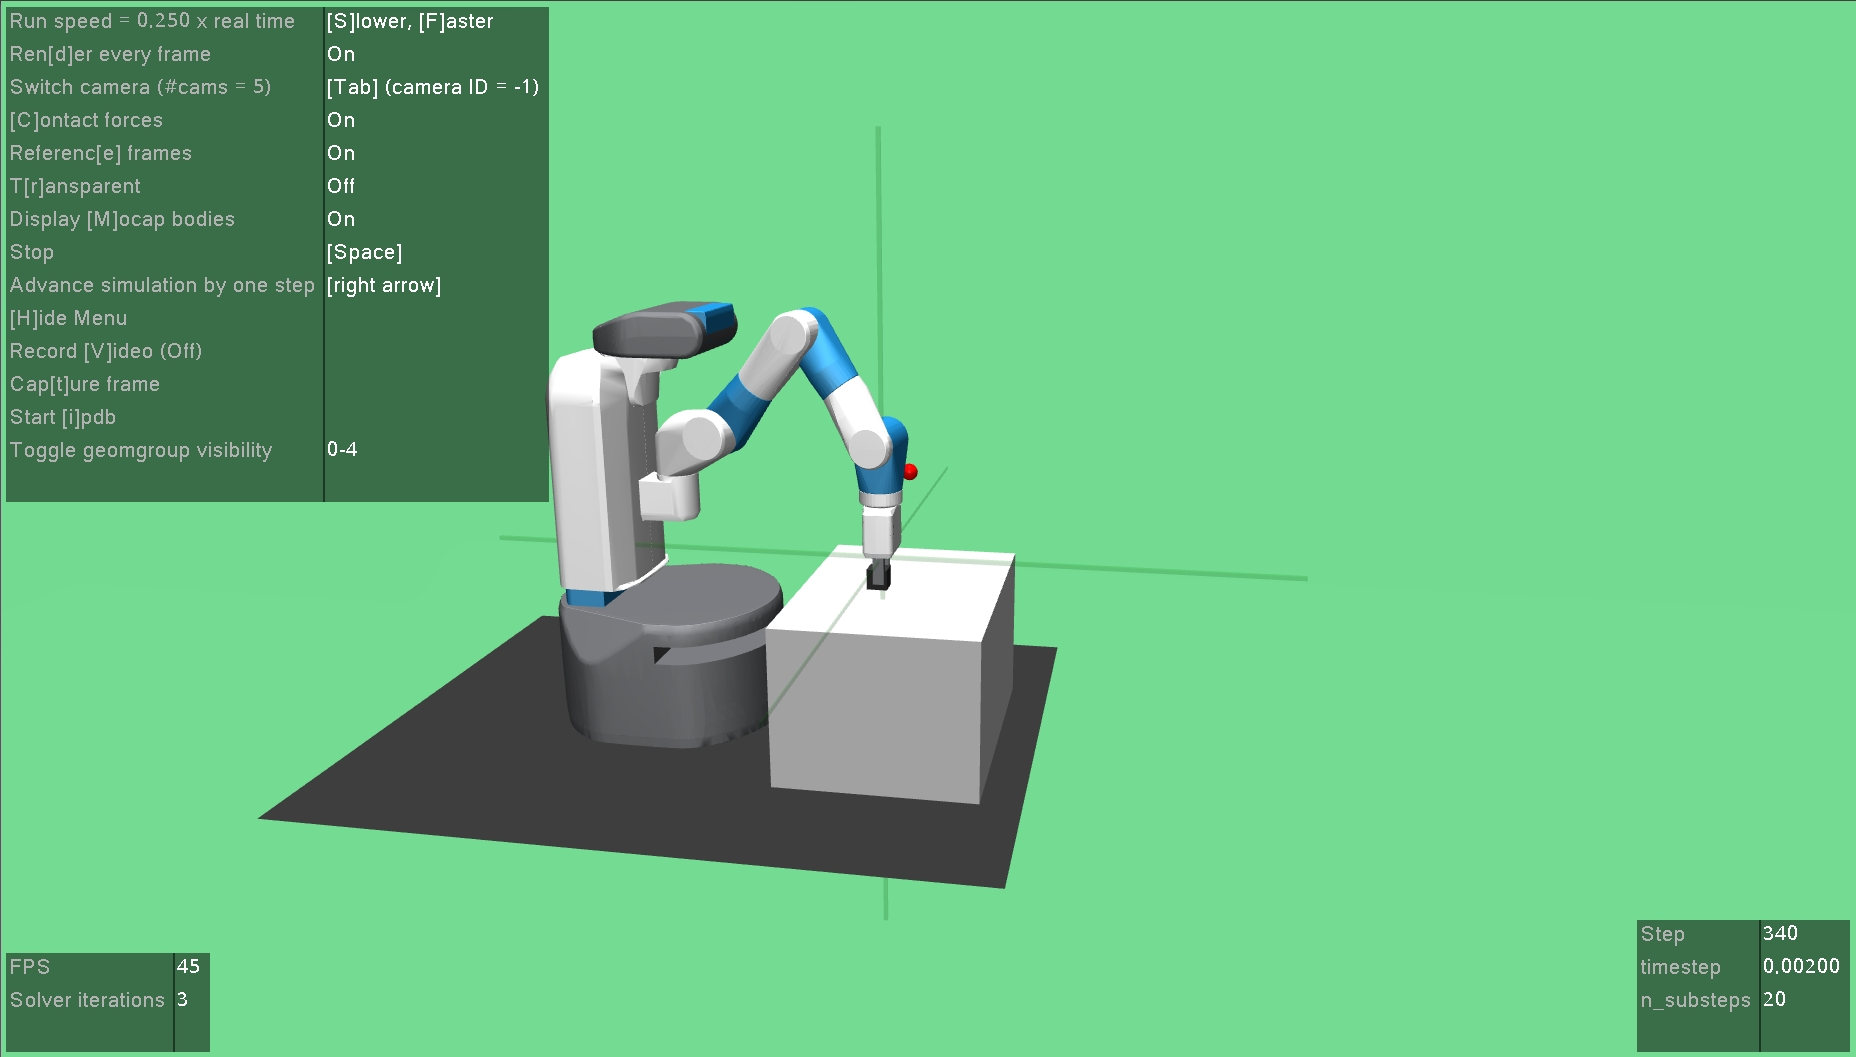
\includegraphics[width=1\textwidth]{figures/FetchPickAndPlace-v1.png}
	\caption{the FetchPickAndPlace-v1 environment by OpenAI Gym run with mujoco-py}
	\label{pickplace1}
\end{figure}

The environment model used is quite simple. The environments are the basic fetch environments in the robotics environment package of OpenAI gym \cite{plappert}, for the extended harder experiments, the object is changed to a ball. Otherwise, only positions of the object and goal as well as properties like size and friction are changed.

\vspace{0.5cm}

In figure \ref{pickplace1} the environment for the task "FetchPickAndPlace" by OpenAI is shown. A fetch robotic arm with 7 DOF is used. Its end effector is a two-fingered parallel gripper. Even though it is simulated in MuJoCo, Andrychowicz et al. have shown in their paper on HER, that the robotic arm also performed well in real life without any finetuning. \cite{herpaper}

\vspace{0.5cm}

All the tasks require an object (either a cube or a ball) to be moved to a goal that is presented by a red point. Also a table is used to increase the height of the object and goal, so the fetch robot can grab the object.
Some parameters except from position parameters that might differ depending on the robotics environment are listed here.

\begin{itemize}
	\item has\_object (boolean): describes whether the environment contains an object or not
	\item block\_gripper (boolean): if True, the fetch robot can not open or close its gripper
	\item n\_substeps (integer): number of timesteps before the next action is chosen
	\item target\_in\_the\_air (boolean): if True, the target is is not on the ground or table 
	\item object\_range (float): defines a range in which the object will be randomly and uniformly placed
	\item target\_range (float): defines the range in which the goal will be randomly and uniformly placed
	\item distance\_threshold (float): the distance the object can be to the goal for the goal to be still successful 
\end{itemize}

In RL, the agent chooses an action and receives a reward and an observation after each step. actions, rewards and observations are handled in OpenAI Gym as follows.

\begin{itemize}
	\item Action: The action space is defined as a 4-dimensional Box space, which is an array of 4 floats, which are continuous and between -1 and 1. The 4 floats define how to change the x-position, y-position and z-position of the gripper and how much to open/close the gripper (if the parameter block\_gripper is False)
	\item Reward: The reward defined as a float. In the robotics environments, the agent receives a reward of -1.0 in each timestep, in which the goal is not reached.
	\item Observation: The observation space contains 3 parts:
	the achieved\_goal, defined by a 3-dimensional Box space, which is useful for HER. 
	the desired\_goal, also defined by a 3-dimensional Box space.
	the observation: defined by a 25-dimnsional Box space
\end{itemize}

If not stated otherwise, each environment sample will be run for 50 steps. With the number of substeps being usually fixed to 20, each sample will run for 1000 timesteps. 
%%use this stuff if it fits

